% Created 2016-09-08 Thu 14:01
% Intended LaTeX compiler: pdflatex
\documentclass[11pt]{article}
\usepackage[utf8]{inputenc}
\usepackage[T1]{fontenc}
\usepackage{graphicx}
\usepackage{grffile}
\usepackage{longtable}
\usepackage{wrapfig}
\usepackage{rotating}
\usepackage[normalem]{ulem}
\usepackage{amsmath}
\usepackage{textcomp}
\usepackage{amssymb}
\usepackage{capt-of}
\usepackage[colorlinks=true, linkcolor=blue]{hyperref}
\usepackage{listings}
\usepackage{multicol}
\usepackage{enumitem}
\setlist[description]{style=nextline}
\usepackage[compact]{titlesec}
\usepackage[landscape,margin=1cm]{geometry}
\titleformat{\section}[frame]
{\normalfont\sffamily}
{\thesection}{.1em}{\small\bfseries\filcenter}
\titleformat{\subsection}[block]
{\normalfont\sffamily}
{\thesection}{0em}{\scriptsize\bfseries\filcenter}
\titleformat{\subsubsection}[block]
{\normalfont\sffamily}
{\thesection}{0em}{\tiny\bfseries}
\pagestyle{empty}
\makeatletter
\renewcommand{\@maketitle}{
\newpage
\begin{center}%
{\Large\bfseries \@title \par}%
\end{center}%
\par}
\makeatother
\setcounter{secnumdepth}{0}
\setlength{\parindent}{0pt}
\setlength{\parskip}{0pt plus 0.5ex}
\lstset{%
basicstyle=\ttfamily\tiny,
commentstyle=\itshape\ttfamily\tiny,
showspaces=false,
showstringspaces=false,
breaklines=true,
breakautoindent=true,
}
\setlist{wide=0pt,nosep}
\usepackage[default,osfigures]{opensans}
\usepackage[scaled=0.8]{luximono}
\date{}
\title{Cheatsheet for YAGS}
\hypersetup{
 pdfauthor={Rafael Villarroel},
 pdftitle={Cheatsheet for YAGS},
 pdfkeywords={},
 pdfsubject={},
 pdfcreator={Emacs 24.5.1 (Org mode N/A)}, 
 pdflang={English}}
\begin{document}

\maketitle
\begin{multicols}{3}
\scriptsize
\thispagestyle{empty}

\section{Graph definitions}
\label{sec:orgde2a8c9}

\begin{description}
\item[{Adjacency list}] \texttt{g:=GraphByAdjacencies([[],[4],[1,2],[]])}

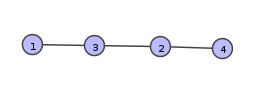
\includegraphics[width=3cm]{bylist.png}
\item[{Adjacency matrix}] \texttt{M:=[[false, true, false], [true, false, true], [false, true, false]];}
\texttt{g:=GraphByAdjMatrix(M);}
\item[{List of edges}] \texttt{g:=GraphByEdges([[1,2],[2,3],[3,4]]);}
\item[{Complete cover}] \texttt{g:=GraphByCompleteCover([[1,2,3,4],[4,5,6]]);}

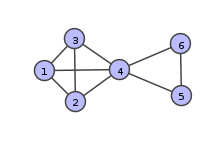
\includegraphics[width=3cm]{bycomplete.png}
\item[{By relation}] \texttt{f:=function(x,y) return Intersection(x,y)<>[]; end;;}
\texttt{g:=GraphByRelation([[1,2,3],[3,4,5],[5,6,7]],f);}
\item[{By walks}] \texttt{g:=GraphByWalks([1,2,3,4,1],[1,5,6]);} 

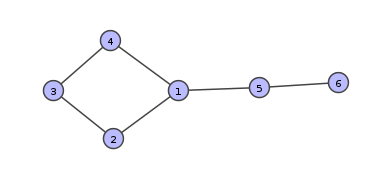
\includegraphics[width=3cm]{bywalks.png}

\texttt{g:=GraphByWalks([1,[2,3,4],5],[5,6]);}

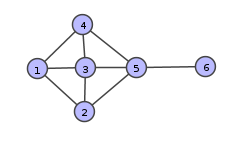
\includegraphics[width=3cm]{bywalks2.png}
\item[{As intersection graph}] \texttt{g:=IntersectionGraph([[1,2,3],[3,4,5],[5,6,7]]);}
\item[{As a copy}] \texttt{h:=CopyGraph(g)}
\item[{As an induced subgraph}] \texttt{h:=InducedSubgraph(g,[3,4,6]);}
\end{description}

\section{Graph families (with parameters)}
\label{sec:org7a55599}

\begin{itemize}
\item \texttt{g:=DiscreteGraph(n)}
\item \texttt{g:=CompleteGraph(n)}
\item \texttt{g:=PathGraph(n)} \(n\) vertices.
\item \texttt{g:=CycleGraph(n)}
\item \texttt{g:=CubeGraph(n)}
\item \texttt{g:=OctahedralGraph(n)}
\item \texttt{g:=JohnsonGraph(n,r)} Vertices are subsets of \(\{1,2,\ldots,n\}\)
with \(r\) elements, edges between subsets with intersection of
\(r-1\) elements.
\item \texttt{g:=Circulant(n,J)} Second paramenter is a list of jumps
\item \texttt{g:=CompleteBipartiteGraph(n,m)}
\item \texttt{g:=CompleteMultipartiteGraph(n1,n2[, n3 ...])}
\item \texttt{g:=TorusGraph(n,m)}
\item \texttt{g:=TreeGraph(L)} \(L\) is a list. Vertices at depth \(k\) have
\texttt{L[k]} children.
\item \texttt{g:=TreeGraph(n,k)} Same as \texttt{TreeGraph([n,n,..,n])} (the list has
length \texttt{k})
\item \texttt{g:=WheelGraph(n)}
\item \texttt{g:=WheelGraph(7,2)} Second optional parameter is the radius of the
wheel.
\item \texttt{g:=FanGraph(4);}
\item \texttt{g:=SunGraph(6);}
\item \texttt{g:=SpikyGraph(4);}
\item Examples: Wheel, Fan, Sun, Spiky:

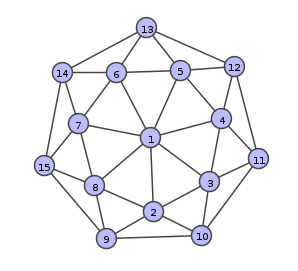
\includegraphics[width=2cm]{wheel.png} 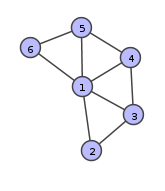
\includegraphics[width=2cm]{fan.png} 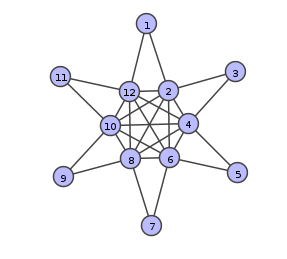
\includegraphics[width=2cm]{sun.png} 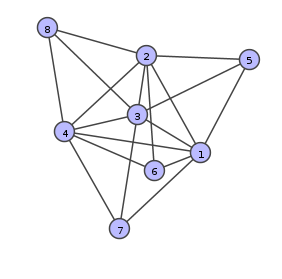
\includegraphics[width=2cm]{spiky.png}
\end{itemize}

\section{Named graphs}
\label{sec:org0852a63}
\begin{description}
\item[{Platonic}] \texttt{Tetrahedron}, \texttt{Octahedron}, \texttt{Cube}, \texttt{Dodecahedron}, \texttt{Icosahedron}.
\item[{Other}] \texttt{TrivialGraph}, \texttt{DiamondGraph}, \texttt{ClawGraph},
\texttt{HouseGraph}, \texttt{BullGraph}, \texttt{AntennaGraph}, \texttt{KiteGraph},
\texttt{AGraph}, \texttt{ChairGraph}, \texttt{DartGraph}, \texttt{DominoGraph},
\texttt{FishGraph}, \texttt{GemGraph}, \texttt{HouseGraph}, \texttt{ParachuteGraph},
\texttt{ParapluieGraph}, \texttt{PawGraph}, \texttt{PetersenGraph}, \texttt{RGraph},
\texttt{SnubDisphenoid}.
\end{description}
\section{Random graphs}
\label{sec:orgd2f50b0}

\begin{itemize}
\item \texttt{g:=RandomGraph(n)}
\item \texttt{g:=RandomGraph(n,p)} Graph with \(n\) vertices, each edge with
probability \(p\) to appear.
\end{itemize}

\section{New graphs from old}
\label{sec:orgba10ae6}

\begin{itemize}
\item \texttt{h:=RemoveVertices(g,[1,3]);}
\item \texttt{h:=AddEdges(g,[[1,2]]);}
\item \texttt{h:=RemoveEdges(g,[[1,2],[3,4]]);}
\end{itemize}

\section{Parameters}
\label{sec:org75df7db}

\begin{itemize}
\item \texttt{Order(g)}
\item \texttt{Size(g)}
\item \texttt{CliqueNumber(g)}
\item \texttt{VertexDegree(g,v)}
\item \texttt{MaxDegree(g)}
\item \texttt{MinDegree(g)}
\item \texttt{Girth(g)}
\item \texttt{NumberOfCliques(g)}
\item \texttt{NumberOfConnectedComponents(g)}
\end{itemize}

\section{Boolean tests}
\label{sec:org6acb5eb}
\begin{itemize}
\item \texttt{IsCompleteGraph(g)}
\item \texttt{IsCliqueHelly(g)}
\item \texttt{IsDiamondFree(g)}
\item \texttt{IsEdge(g,x,y)} or \texttt{IsEdge(g,[x,y])}
\item \texttt{IsIsomorphicGraph(g,h)}
\item \texttt{IsCompactSurface(g)}
\item \texttt{IsSurface(g)}
\item \texttt{IsLocallyConstant(g)}
\item \texttt{IsLocallyH(g,h)}
\item \texttt{IsLoopless(g)}
\end{itemize}

\section{Products}
\label{sec:orgcba1cc0}
\begin{itemize}
\item \texttt{p=BoxProduct(g,h)}
\item \texttt{p=TimesProduct(g,h)}
\item \texttt{p=BoxTimesProduct(g,h)}
\item \texttt{p=DisjointUnion(g,h)}
\item \texttt{p=Join(g,h)}
\item \texttt{p=GraphSum(g,l)} \(l\) is a list of graphs. Suppose that \(g\) has
\(n\) vertices. In the disjoint union of the first \(n\) graphs of
\(l\) (using \texttt{TrivialGraphs} if needed to fill \(n\) slots), add all
edges between graphs corresponding to adjacent vertices in \(g\).
\item \texttt{p=Composition(g,h)} is the same as \texttt{GraphSum(g,l)}, where \(l\) is
a list of length the order of \(g\), with all components equal to
\(h\).
\end{itemize}

\section{Operators}
\label{sec:org1ce4b76}

\begin{itemize}
\item \texttt{h:=CliqueGraph(g)}
\item \texttt{h:=CliqueGraph(g,m)} Stops when a maximum of
\(m\) cliques have been found.
\item \texttt{h:=LineGraph(g)}
\item \texttt{h:=ComplementGraph(g)}
\item \texttt{h:=Cone(g)}
\item \texttt{h:=Suspension(g)}
\item \texttt{h:=ParedGraph(g)}
\item \texttt{h:=CompletelyParedGraph(g)}
\item \texttt{h:=QuotientGraph(g,p)} \(p\) is a partition of vertices. The
vertices of \(h\) are the parts of \(p\), with two vertices adjacent
if there are two vertices adjacent in \(g\) in the corresponding
parts. Singletons in \(p\) may be omitted.
\item \texttt{h:=QuotientGraph(g,l1,l2)} \(l1,l2\) are lists of vertices of the
same length, with repetitions allowed. In \(h\), each vertex of the
first list is identified with the corresponding vertex in the second
list.
\item \texttt{h:=Link(g,x)} The subgraph of \(g\) induced by the neighbors of
\(x\).
\item \texttt{h:=SpanningForest(g)}
\end{itemize}

\section{Lists}
\label{sec:orga9787f5}
\begin{itemize}
\item \texttt{VertexNames(g)}
\item \texttt{Cliques(g)}
\item \texttt{Cliques(g,m)} Stops if a maximum of \(m\) cliques have been found.
\item \texttt{Basement(kng,kmg,x)} \(n\leq m\)
\item \texttt{AdjMatrix(g)}
\item \texttt{Adjaceny(g,v)}
\item \texttt{Adjacencies(g)}
\item \texttt{VertexDegrees(g)}
\item \texttt{Edges(g)}
\item \texttt{CompletesOfGivenOrder(g,o)}
\item \texttt{ConnectedComponents(g)}
\item \texttt{GraphAttributeStatistics(n,p,F)} Returns information about the
parameter \texttt{F} for 100 random graphs of order \(n\) and edge
probability \(p\).
\item \texttt{BoundaryVertices(g)} For \(g\) a triangulation of a compact
surface, returns the list of vertices whose link is isomorphic to a
path.
\item \texttt{InteriorVertices(g)}
\item \texttt{SpanningForestEdges(g)}
\end{itemize}

\section{Distances}
\label{sec:org56e38cd}
\begin{itemize}
\item \texttt{Distance(g,x,y)}
\item \texttt{DistanceMatrix(g)}
\item \texttt{Diameter(g)}
\item \texttt{Eccentricity(g,x)}
\item \texttt{Radius(g)}
\item \texttt{Distances(g,a,b)} \(a\), \(b\) are lists of vertices. Returns a list.
\item \texttt{DistanceSet(g,a,b)} As before, but returns a set.
\item \texttt{DistanceGraph(g,d)} The graph with vertex set the vertices of
\(g\), two vertices adjacent if their distance is in \(d\).
\item \texttt{PowerGraph(g,n)} Same as the distance graph with set of distance
\(\{1,\ldots,n\}\).
\end{itemize}

\section{Graph morphisms}
\label{sec:orgfd8b47d}

\begin{itemize}
\item \texttt{IsoMorphisms(g,h)}
\item \texttt{AutomorphismGroup(g)}
\item \texttt{Morphism(g,h)}, \texttt{Morphisms(g,h)}, \texttt{NextMorphism(g,h,f)}
\item \texttt{MonoMorphism(g,h)}, \texttt{MonoMorphisms(g,h)}, \texttt{NextMonoMorphism(g,h,f)}
\item \texttt{EpiMorphism(g,h)}, \texttt{EpiMorphisms(g,h)}, \texttt{NextEpiMorphism(g,h,f)}
\item \texttt{WeakMorphism(g,h)}, \texttt{WeakMorphisms(g,h)},
\texttt{NextWeakMorphism(g,h,f)}, and more predefined classes of morphisms and the
possibility to define new classes
\end{itemize}

\section{Small Graphs}
\label{sec:org9a84729}

\begin{itemize}
\item \texttt{ConnectedGraphsOfGivenOrder(n)} Up to \(n=9\).
\item \texttt{Graph6ToGraph(s)} \texttt{s} is a string.
\item \texttt{GraphsOfGivenOrder(n)} Up to \(n=9\).
\item \texttt{ImportGraph6(f)} \texttt{f} is a filename.
\end{itemize}

\section{Graph categories}
\label{sec:org80b9746}

\begin{itemize}
\item \texttt{DefaultGraphCategory} A variable that holds the current graph
category. Has to be set with, e.g. \texttt{SetDefaultCategory(OrientedGraphs)}
\end{itemize}

\subsection{Graph categories:}
\label{sec:org21f9056}
\texttt{Graphs}, \texttt{UndirectedGraphs}, \texttt{LooplessGraphs}, \texttt{SimpleGraphs},
\texttt{OrientedGraphs}. 

\section{Digraphs}
\label{sec:org972a7a3}

\begin{itemize}
\item \texttt{InNeigh(g,x)} List of in-neighbors of \(x\) in \(g\).
\item \texttt{IsTournament(g)}
\item \texttt{IsTransitiveTournament(g)}
\item \texttt{Orientations(g)} List of all oriented graphs that can be obtained
from \(g\)
\end{itemize}

\section{Draw}
\label{sec:org84111ef}
\begin{itemize}
\item \texttt{Draw(g)} Shows a window with a drawing of \texttt{g}. Commands in the \texttt{draw} window: \texttt{h}:help, \texttt{f}:fit graph,
\texttt{l}: toggle labels, \texttt{d}: toggle dynamics, \texttt{r}: toggle repulsion, \texttt{s}: save \& quit, \texttt{q}:
quit without saving
\end{itemize}

\section{Backtrack}
\label{sec:org809335c}

Example: coloring with two colors:
\lstset{basicstyle=\ttfamily,commentstyle=\itshape\ttfamily\color{green!50!black},keywordstyle=\bfseries\color{blue},stringstyle=\color{purple},breaklines=true,showstringspaces=false,language=gap,label= ,caption= ,captionpos=b,numbers=none}
\begin{lstlisting}
g:=PathGraph(3);
chk:=function(L,g)
    local x,y;
    if L=[] then return true; fi;
    x:=Length(L);
    for y in [1..x-1] do
        if IsEdge(g,[x,y]) and L[x]=L[y] then
            return false;
        fi;
    od;
    return true;
end;
\end{lstlisting}
then \texttt{BacktrackBag([0,1],chk,Order(g),g);} returns \texttt{[ [ 0, 1, 0 ], [
  1, 0, 1 ] ]}. 


\end{multicols}
\end{document}